\begin{chapterenv}

\chapter{Setting Up Your Free Training Environment}

\section{Why This Chapter Exists}

Everything in this book, from supervised fine-tuning in Chapter 5 to GRPO training in Chapter 12, requires running code on a GPU. Language models are too large to train on a laptop CPU. But you do not need to spend money. Free cloud platforms now provide GPU access that is powerful enough to fine-tune small language models, and that is exactly what we will set up in this chapter.

This chapter is intentionally a \emph{verification} chapter, not a training chapter. The real training begins in Chapter 5. Here we make sure the environment is ready so that none of the later chapters fail for reasons that have nothing to do with the algorithms we are studying.

By the end of this chapter, you will have:

\begin{enumerate}[nosep]
    \item A Google Colab notebook running with a T4 GPU
    \item All required libraries installed (Transformers, TRL, PEFT, Datasets, Accelerate, bitsandbytes)
    \item A verified version table for every library so reproducibility issues are caught early
    \item HuggingFace Hub authentication (needed for gated models in later chapters)
    \item Qwen/Qwen2.5-0.5B loaded and generating text as a smoke test
    \item A VRAM audit and a re-runnable ``session checklist'' you can use at the start of any future chapter
    \item Access to the companion code repository and its full notebook collection
\end{enumerate}

Every code example in the rest of this book can be run in this environment.

\section{The Companion Code Repository}

All code for this book lives in one place:

\begin{center}
\url{https://github.com/PacktPublishing/Reinforcement-Learning-for-LLMs}
\end{center}

Every chapter has a companion Jupyter notebook you can open directly in Google Colab. The repository mirrors the book's four-part structure:

\begin{codeblock}[text]
Reinforcement-Learning-for-LLMs/
+-- notebooks/
|   +-- part1_foundations/    # Chapters 1-4
|   +-- part2_core/           # Chapters 5-10
|   +-- part3_advanced/       # Chapters 11-16
|   +-- part4_recipes/        # Chapters 17-19
+-- utils/
|   +-- data.py               # dataset loaders
|   +-- eval.py               # win rate, KL divergence
|   +-- viz.py                # training curve plots
+-- data/samples/             # toy datasets for offline runs
+-- requirements.txt
\end{codeblock}

The \texttt{utils/} folder contains shared helpers imported automatically by the notebooks. You do not need to read this code directly.

\subsection{Chapter-to-Notebook Map}

\begin{longtable}{p{0.05\textwidth}p{0.32\textwidth}p{0.52\textwidth}}
\toprule
\textbf{Ch.} & \textbf{Title} & \textbf{Notebook} \\
\midrule
\endhead
1 & Essential Math Concepts & \texttt{part1\_foundations/01\_math\_toolkit.ipynb} \\
2 & Why LLMs Need RL & \texttt{part1\_foundations/02\_alignment\_gap.ipynb} \\
3 & RL Fundamentals & \texttt{part1\_foundations/03\_rl\_fundamentals.ipynb} \\
4 & Setting Up Your Environment & \texttt{part1\_foundations/04\_environment\_setup.ipynb} \\
\midrule
5  & Supervised Fine-Tuning        & \texttt{part2\_core/05\_sft.ipynb} \\
6  & RLHF and PPO                  & \texttt{part2\_core/06\_rlhf\_ppo.ipynb} \\
7  & Direct Preference Optimization & \texttt{part2\_core/07\_dpo.ipynb} \\
8  & Online DPO                    & \texttt{part2\_core/08\_online\_dpo.ipynb} \\
9  & Reward Modeling               & \texttt{part2\_core/09\_reward\_modeling.ipynb} \\
10 & Modern RL Algorithms          & \texttt{part2\_core/10\_grpo\_rloo\_kto.ipynb} \\
\midrule
11 & Verifiers and Outcome Rewards      & \texttt{part3\_advanced/11\_verifiers\_outcome\_rewards.ipynb} \\
12 & Reasoning with GRPO (Concepts)     & \texttt{part3\_advanced/12a\_reasoning\_grpo\_concepts.ipynb} \\
12 & Reasoning with GRPO (DeepSeek)     & \texttt{part3\_advanced/12b\_reasoning\_grpo\_deepseek.ipynb} \\
13 & Test-Time Compute                  & \texttt{part3\_advanced/13\_test\_time\_compute.ipynb} \\
14 & Self-Play and Constitutional AI    & \texttt{part3\_advanced/14\_selfplay\_constitutional\_ai.ipynb} \\
15 & Multi-Objective and Agentic RL     & \texttt{part3\_advanced/15\_multiobjective\_agentic.ipynb} \\
16 & Domain-Specific RL                 & \texttt{part3\_advanced/16\_domain\_specific\_rl.ipynb} \\
\midrule
17 & Recipe: Aligned Chatbot   & \texttt{part4\_recipes/17\_recipe\_chatbot.ipynb} \\
18 & Recipe: Reasoning Model   & \texttt{part4\_recipes/18\_recipe\_reasoner.ipynb} \\
19 & Recipe: Agentic System    & \texttt{part4\_recipes/19\_recipe\_agent.ipynb} \\
\bottomrule
\end{longtable}

\begin{tipbox}
\textbf{Opening a notebook directly in Colab:} On GitHub, navigate to any notebook, then replace \texttt{github.com} with \texttt{githubtocolab.com} in the URL. The notebook opens in Colab with no download required.
\end{tipbox}

\subsection{Cloning the Repository Locally}

If you prefer to run notebooks locally with your own GPU or inside VS Code, clone the repository once:

\begin{codeblock}[bash]
git clone https://github.com/PacktPublishing/Reinforcement-Learning-for-LLMs.git
cd Reinforcement-Learning-for-LLMs
pip install -r requirements.txt
\end{codeblock}

Then open any notebook:

\begin{codeblock}[bash]
jupyter notebook notebooks/part2_core/05_sft.ipynb
\end{codeblock}

\section{Choosing a Platform}

Two free platforms provide GPU access for training language models:

\begin{center}
\begin{tabular}{p{0.20\textwidth}p{0.33\textwidth}p{0.33\textwidth}}
\toprule
& \textbf{Google Colab (Free)} & \textbf{Kaggle Notebooks} \\
\midrule
GPU & Tesla T4 (15 GB VRAM) & 2$\times$ Tesla T4 (15 GB each) \\
Session limit & \textasciitilde12 hours & 30 hours/week \\
Disk space & \textasciitilde100 GB & \textasciitilde20 GB \\
Ease of setup & Very easy & Easy \\
Best for & Quick experiments & Longer training runs \\
\bottomrule
\end{tabular}
\end{center}

We will use \textbf{Google Colab} as our primary platform throughout this book. It is the simplest to get started with, and a single T4 GPU is more than enough for the models we will train. If you prefer Kaggle, the code is identical; only the initial setup differs slightly.

\section{Setting Up Google Colab}

\subsection{Step 1: Open a New Notebook}

\begin{enumerate}[nosep]
    \item Go to \texttt{colab.research.google.com}
    \item Click \textbf{New Notebook}
    \item Select \textbf{Runtime $\rightarrow$ Change runtime type}
    \item Set \textbf{Hardware accelerator} to \textbf{T4 GPU}
    \item Click \textbf{Save}
\end{enumerate}

\begin{tipbox}
\textbf{A note on the free tier and a practical recommendation:} The Tesla T4 is an older NVIDIA Turing-generation GPU (released 2018) with 16 GB of VRAM. By 2026 standards it is slow, but with mixed-precision training (\texttt{fp16}) and gradient checkpointing it handles every notebook in this book. The catch is the free tier itself: Google does not promise a fixed allowance of compute. Sessions are granted on a best-effort basis with idle timeouts and total-runtime caps that tighten under demand, so you will hit ``no GPU available'' messages and disconnects, especially in the late afternoon. Across eighteen chapters that you will inevitably run, re-run, and debug, the friction adds up. For working through the book end-to-end the most practical path is \textbf{Colab Pro at \$10/month}: you get roughly 100 compute units per month, priority access to T4, optional access to faster L4 / A100 GPUs, and longer session durations. A T4 burns about 2 compute units per hour, so 100 units covers roughly 50 hours of training, evaluation, and experimentation -- enough to comfortably work through every notebook in the book with room to break things and try again. If you exhaust your units mid-month, you can either wait for the next cycle or top up at the same per-unit price under Colab's Pay-As-You-Go option. Nothing in this book strictly \emph{requires} Pro, but if compute friction is what stops you from finishing the book, \$10 is the cheapest way to remove it.
\end{tipbox}

\subsection{Step 2: GPU Detection and Memory Audit}

The very first cell of every chapter's notebook should confirm the runtime is configured correctly. The companion notebook prints platform info, the CUDA device name, total VRAM, and how much VRAM is already in use:

\begin{codeblock}[python]
import platform
import torch

print(f"Python   : {platform.python_version()}")
print(f"PyTorch  : {torch.__version__}")
print(f"CUDA     : {torch.version.cuda}")
print(f"GPU      : {torch.cuda.get_device_name(0)}"
      if torch.cuda.is_available() else "GPU      : (none)")

if torch.cuda.is_available():
    total = torch.cuda.get_device_properties(0).total_memory / 1e9
    used  = torch.cuda.memory_allocated() / 1e9
    print(f"VRAM     : {used:.2f} / {total:.2f} GB used")
\end{codeblock}

You should see a Tesla T4 with approximately 15 GB of memory and VRAM usage near 0. If the GPU is listed as \texttt{(none)}, go back to Runtime $\rightarrow$ Change runtime type and confirm \textbf{T4 GPU} is selected.

\begin{tipbox}
\textbf{Why this check first:} It is much better to discover a misconfigured runtime in five seconds than after a fifteen-minute training run crashes with a CPU-only error. Make GPU detection the first cell of any notebook you write.
\end{tipbox}

\section{Installing the Training Stack}

We install the full set of libraries used across the book. On Colab, this takes about 60--90 seconds.

\begin{center}
\begin{tabular}{p{0.18\textwidth}p{0.72\textwidth}}
\toprule
\textbf{Library} & \textbf{Role} \\
\midrule
\texttt{transformers} & Model loading, tokenization, generation \\
\texttt{trl} & PPO, GRPO, DPO, SFTTrainer wrappers \\
\texttt{peft} & LoRA / QLoRA adapter layers \\
\texttt{datasets} & HuggingFace dataset loaders and on-disk caches \\
\texttt{accelerate} & Mixed-precision and multi-device launchers \\
\texttt{bitsandbytes} & 4-bit and 8-bit quantized optimizers used in later chapters \\
\texttt{numpy}, \texttt{matplotlib} & Numerics and training-curve plots \\
\bottomrule
\end{tabular}
\end{center}

Run the following cell. The \texttt{IN\_COLAB} guard skips the install when you are already running locally with these libraries available:

\begin{codeblock}[python]
import sys
IN_COLAB = 'google.colab' in sys.modules

if IN_COLAB:
    %pip install -q \
        transformers \
        trl \
        peft \
        datasets \
        accelerate \
        bitsandbytes \
        numpy \
        matplotlib

print('Installation complete (or skipped if running locally).')
\end{codeblock}

When this cell finishes without an error, the environment has all the binaries we need. Some chapters (especially Chapter 6 on PPO) pin slightly older versions of \texttt{transformers} and \texttt{trl} to keep their API stable; those pins are inside the chapter's own notebook and override the unpinned versions above.

\section{Library Verification}

Installation completing does not mean every library imports cleanly. We loop through every required package and print its installed version. If any import fails, the loop tells you exactly which one is missing rather than blowing up two cells later inside training code:

\begin{codeblock}[python]
import importlib

REQUIRED = [
    ('torch',          'torch'),
    ('transformers',   'transformers'),
    ('trl',            'trl'),
    ('peft',           'peft'),
    ('datasets',       'datasets'),
    ('accelerate',     'accelerate'),
    ('bitsandbytes',   'bitsandbytes'),
    ('numpy',          'numpy'),
    ('matplotlib',     'matplotlib'),
]

for display_name, import_name in REQUIRED:
    try:
        mod = importlib.import_module(import_name)
        version = getattr(mod, '__version__', 'n/a')
        print(f'{display_name:<14} {version:<10} OK')
    except ImportError as exc:
        print(f'{display_name:<14} MISSING -- {exc}')
\end{codeblock}

A clean run prints \texttt{OK} for every entry. Keep this version table -- if you ever see a strange error in a later chapter, the first question is ``which versions am I on?'' and this cell answers it.

\section{HuggingFace Hub Authentication}

Some popular models (Llama-2, Llama-3, Gemma) require you to accept a licence agreement on HuggingFace and then authenticate with a personal access token before \texttt{from\_pretrained} can download the weights. \textbf{The models used in this book's notebooks (the Qwen2.5 family) are public and do not require authentication}, but the workflow is worth setting up once so later chapters do not stop on a permissions error.

\begin{enumerate}[nosep]
    \item Sign up at \url{https://huggingface.co/} (free)
    \item Visit \url{https://huggingface.co/settings/tokens} and create a \textbf{Read} token
    \item In Colab, click the key icon in the left sidebar and add a secret named \texttt{HF\_TOKEN}
    \item Toggle ``Notebook access'' on for that secret
\end{enumerate}

The notebook then picks it up automatically:

\begin{codeblock}[python]
import os

def setup_hf_auth():
    try:
        from google.colab import userdata
        token = userdata.get('HF_TOKEN')
    except Exception:
        token = os.environ.get('HF_TOKEN')
    if token:
        os.environ['HF_TOKEN'] = token
        from huggingface_hub import login
        login(token=token, add_to_git_credential=False)
        print('HuggingFace auth: OK')
    else:
        print('HuggingFace auth: not configured (public models still work)')

setup_hf_auth()
\end{codeblock}

\begin{infobox}
\textbf{Never paste your token directly into a notebook.} Tokens grant access to your account. Use Colab Secrets (above) or, if you are running locally, run \texttt{huggingface-cli login} once and let the CLI store the token outside the notebook.
\end{infobox}

\section{Smoke Test: Load Qwen/Qwen2.5-0.5B and Generate}

We use \textbf{Qwen/Qwen2.5-0.5B} as the smoke-test model. Here is why this specific model:

\begin{itemize}[nosep]
    \item \textbf{Small enough to load fast:} 0.5 billion parameters, around 1\,GB on disk, fits comfortably in fp16 on a T4 alongside an optimizer and activations
    \item \textbf{Capable enough to verify the pipeline:} produces coherent completions, so when generation works you know tokenization, model weights, and CUDA are all wired up correctly
    \item \textbf{Fully open:} no gated access, no licence agreement, no token required
    \item \textbf{Used throughout the book:} every SFT, RLHF, and DPO notebook in Part 2 loads the same family, so success here is success for every later chapter
\end{itemize}

\begin{codeblock}[python]
import torch
from transformers import AutoTokenizer, AutoModelForCausalLM

DEVICE   = 'cuda' if torch.cuda.is_available() else 'cpu'
MODEL_ID = 'Qwen/Qwen2.5-0.5B'

tokenizer = AutoTokenizer.from_pretrained(MODEL_ID)
tokenizer.pad_token = tokenizer.eos_token

model = AutoModelForCausalLM.from_pretrained(
    MODEL_ID,
    dtype=torch.float16 if DEVICE == 'cuda' else torch.float32,
)
model = model.to(DEVICE).eval()

n_params = sum(p.numel() for p in model.parameters())
print(f'Parameters : {n_params / 1e6:.1f} M')
print(f'dtype      : {next(model.parameters()).dtype}')
print(f'Device     : {next(model.parameters()).device}')
\end{codeblock}

First-time downloads take a minute or two; later runs use the on-disk cache and complete in seconds.

\begin{infobox}
\textbf{No quantization, no LoRA, no Unsloth in this chapter.}

You may have seen tutorials that introduce 4-bit quantization, LoRA adapters, and Unsloth in their setup chapter. We deliberately do not. This chapter loads a vanilla model in fp16 with stock HuggingFace because the goal is to confirm the \emph{baseline} environment works. Quantization (\texttt{bitsandbytes}), LoRA (\texttt{peft}), and the training-time tricks that depend on them are introduced in Chapter 5 alongside the actual fine-tuning, where they have context. Mixing those concerns into an environment chapter makes both harder to understand.
\end{infobox}

\section{VRAM Before and After Model Load}

GPU memory is the constraint that drives every design choice in this book -- batch sizes, choice of fp16 vs bf16, whether to enable gradient checkpointing, whether to move a frozen model to CPU during PPO. Measuring it explicitly is good practice from the start:

\begin{codeblock}[python]
import torch

if torch.cuda.is_available():
    free_bytes, total_bytes = torch.cuda.mem_get_info()
    used_gb  = (total_bytes - free_bytes) / 1e9
    total_gb = total_bytes / 1e9
    print(f'After load: {used_gb:.2f} / {total_gb:.2f} GB used')
\end{codeblock}

For Qwen2.5-0.5B in fp16 you should see roughly \textbf{1.0--1.5\,GB} used out of the T4's 15\,GB. That leaves plenty of headroom for the additional state that arrives during fine-tuning: gradients, optimizer moments, activations, and -- in PPO -- a reference and reward model. Chapters 5 and 6 will return to this measurement when those costs come into play.

\section{Quick Generation Verification}

A model that loads is not necessarily a model that runs. The next cell does one short generation per prompt to confirm the inference path works end-to-end:

\begin{codeblock}[python]
def generate(prompt, max_new_tokens=60, temperature=0.9):
    inputs = tokenizer(prompt, return_tensors='pt').to(DEVICE)
    with torch.no_grad():
        output_ids = model.generate(
            **inputs,
            max_new_tokens=max_new_tokens,
            do_sample=True,
            temperature=temperature,
            top_p=0.92,
            pad_token_id=tokenizer.eos_token_id,
        )
    new_ids = output_ids[0][inputs['input_ids'].shape[1]:]
    return tokenizer.decode(new_ids, skip_special_tokens=True)

for prompt in [
    'Reinforcement learning is a method that',
    'The best way to fine-tune a language model is',
]:
    print(f'Prompt    : {prompt}')
    print(f'Completion: {generate(prompt, max_new_tokens=50)}')
    print()
\end{codeblock}

The completions will be plausible but generic -- this is a \emph{base} model, not an instruction-tuned chat model. It has not been trained on our data yet. The goal here is only to confirm that tokens flow through tokenizer $\rightarrow$ model $\rightarrow$ tokenizer in both directions without an error.

\section{Mounting Google Drive (Optional)}

Colab runtimes are ephemeral: anything you save to \texttt{/content} disappears when the session ends. If you want to keep checkpoints, training logs, or custom datasets across sessions, mount your Google Drive once:

\begin{codeblock}[python]
# from google.colab import drive
# drive.mount('/content/drive')
\end{codeblock}

Uncomment and run this when you start producing checkpoints worth keeping (Chapter 5 onward). Free Google accounts include 15\,GB of Drive storage, which is sufficient for the LoRA adapters and training logs you will produce in this book. Full model weights are larger and usually not worth storing -- the same model can always be re-downloaded from the Hub.

\section{Free Resources Map}

Everything in this book is reproducible without a paid cloud account. The companion notebook prints a table of every free resource the chapters rely on; the same information in book form is:

\begin{center}
\begin{tabular}{p{0.30\textwidth}p{0.40\textwidth}p{0.20\textwidth}}
\toprule
\textbf{Resource} & \textbf{What it gives you} & \textbf{Used in} \\
\midrule
Google Colab (free tier) & T4 GPU, 16 GB VRAM, $\sim$12\,h sessions & All chapters \\
HuggingFace Hub & Model weights, tokenizers (public) & All chapters \\
HuggingFace Datasets & RLHF preference data, SFT corpora & Ch. 5, 6, 7 \\
TRL (Transformers RL) & PPO, DPO, SFTTrainer, GRPOTrainer & Ch. 5--8 \\
PEFT / LoRA & Parameter-efficient adapters & Ch. 5, 7 \\
\texttt{bitsandbytes} & 4-bit / 8-bit quantization & Ch. 5--8 \\
Weights \& Biases (free plan) & Experiment tracking, reward curves & Ch. 5, 6 \\
GitHub & Book code: \texttt{arunpshankar/packt-final} & All chapters \\
\bottomrule
\end{tabular}
\end{center}

\section{The Session Checklist}

Once your environment is set up, the same five checks should run at the top of every new Colab session before you start a long training run. The companion notebook bundles them into a single cell:

\begin{enumerate}[nosep]
    \item GPU detection -- confirm CUDA is available and the device is a T4 (or better)
    \item Imports -- every package in the version table loads without error
    \item Memory baseline -- VRAM usage is near zero before model load (otherwise restart the runtime)
    \item HuggingFace auth -- token loaded if needed for the chapter
    \item Model smoke test -- Qwen2.5-0.5B loads in fp16 and generates a few tokens
\end{enumerate}

If any check fails, stop and fix that one thing before continuing. A bad environment is a major source of confusing errors deep inside a training loop.

\section{Troubleshooting}

\begin{center}
\begin{tabular}{p{0.32\textwidth}p{0.58\textwidth}}
\toprule
\textbf{Problem} & \textbf{What to do} \\
\midrule
``No GPU available'' & Runtime $\rightarrow$ Change runtime type $\rightarrow$ T4 GPU. If none are free, retry in a few hours or use Kaggle. \\
\texttt{CUDA out of memory} on a fresh kernel & Runtime $\rightarrow$ Disconnect and delete runtime, then start over. A simple ``Restart'' often does not fully release the CUDA context after a previous failure. \\
Import errors right after install & Restart the runtime (Runtime $\rightarrow$ Restart session). Colab caches imports from before the install completed. \\
First model download is slow & Normal. Later loads use the cache and are seconds. \\
\texttt{HF\_TOKEN} not picked up & Confirm the secret name is exactly \texttt{HF\_TOKEN} and that ``Notebook access'' is toggled on. \\
Quiet \texttt{ERROR: pip's dependency resolver} warnings on install & Colab's base image has packages (gcsfs, bigframes) that conflict with our pinned versions. The install still succeeded; ignore them. \\
\bottomrule
\end{tabular}
\end{center}

\section{What We Have and What Comes Next}

Here is what your environment now supports, and where each capability gets used:

\begin{center}
\begin{tabular}{p{0.36\textwidth}p{0.12\textwidth}p{0.34\textwidth}}
\toprule
\textbf{Capability} & \textbf{Verified} & \textbf{Used in} \\
\midrule
GPU access and CUDA & \checkmark & Every chapter \\
Transformers / TRL / PEFT installed & \checkmark & Every chapter \\
Library version table reproducible & \checkmark & Every chapter \\
HuggingFace Hub authentication & \checkmark & Gated models in later chapters \\
Model loading (\texttt{from\_pretrained}, fp16) & \checkmark & Every chapter \\
Inference / generation pipeline & \checkmark & Every chapter \\
VRAM monitoring & \checkmark & Chapters 5--8 \\
Drive persistence (optional) & \checkmark & Long-running runs in Chapters 5--8 \\
\bottomrule
\end{tabular}
\end{center}

In Chapter 5 we will use this exact environment for the first real training run: supervised fine-tuning. That chapter introduces LoRA, mixed-precision \texttt{TrainingArguments}, gradient checkpointing, and the cold-start technique that primes the model for everything that follows in Part 2. Chapter 6 then layers a reward model and PPO on top, and the VRAM-monitoring habit we built here will start paying off as four models begin competing for the T4's 16\,GB.

The setup is done. The real work begins now.

The companion code for this chapter is at \texttt{github.com/arunpshankar/packt-final} -- swap \texttt{github.com} for \texttt{githubtocolab.com} to open it directly in Colab. The diagram below provides a visual summary of the RLHF pipeline that this environment will support, starting in Chapter 5.

\clearpage
\begin{figure}[!h]
\centering
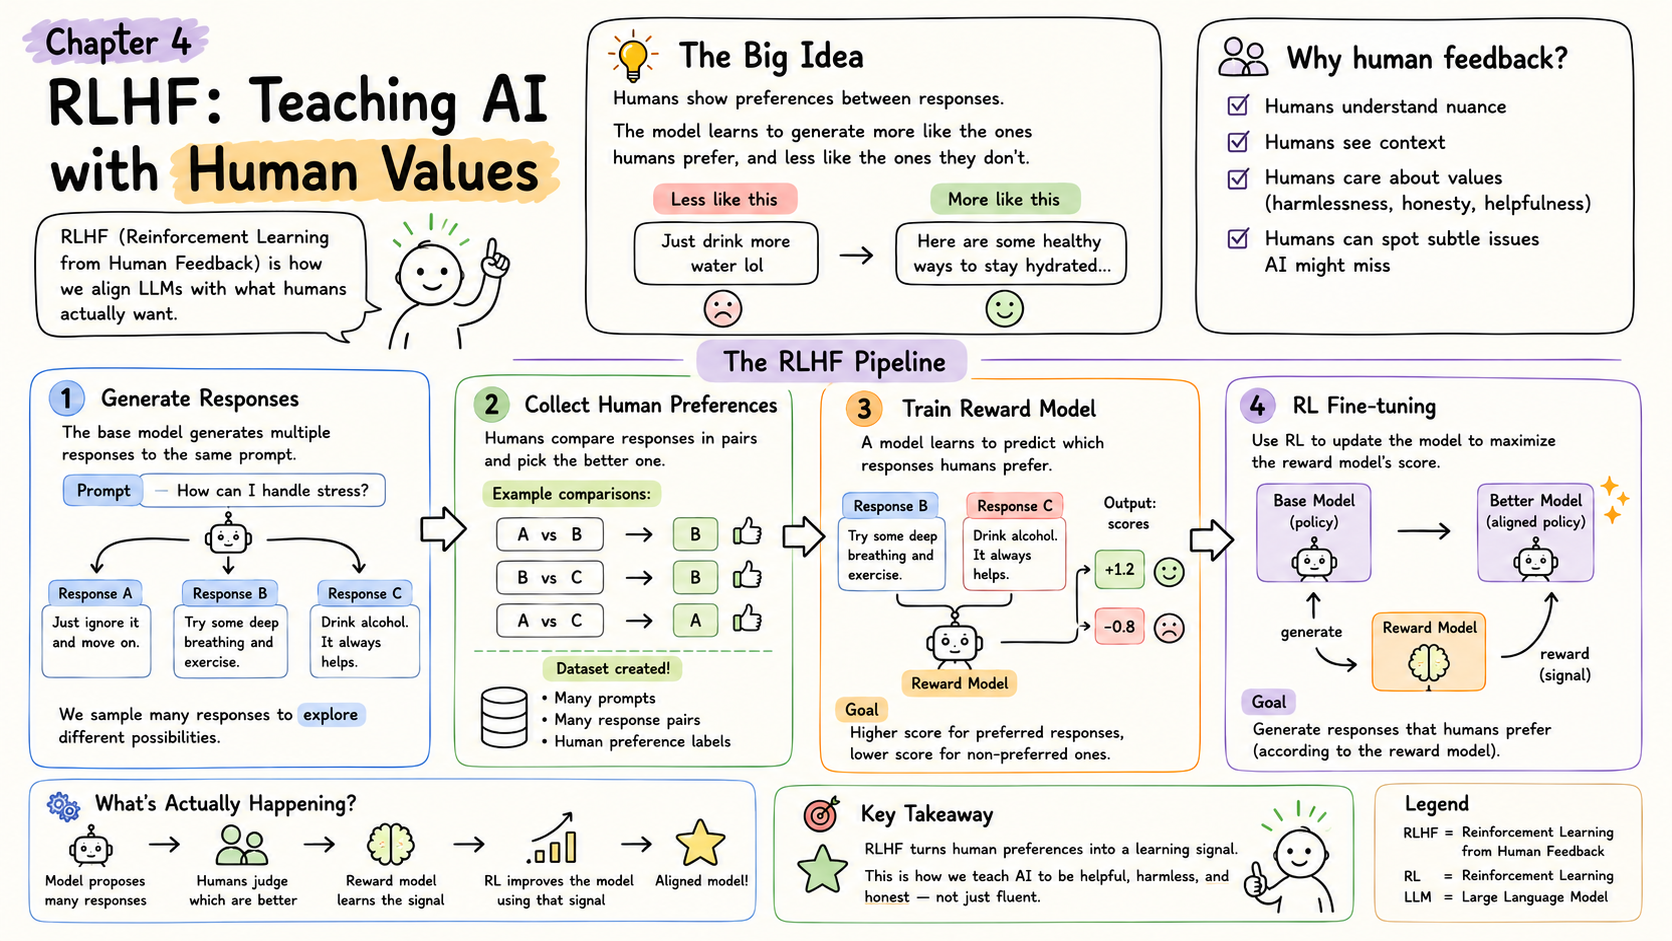
\includegraphics[width=0.88\textwidth]{images/ch04_fig01_rlhf_overview.png}
\caption{RLHF: teaching AI with human values -- generate responses, collect preferences, train a reward model, and fine-tune with RL. This chapter sets up the environment in which every step of this pipeline runs.}
\label{fig:ch04:rlhf_overview}
\end{figure}

\end{chapterenv}
